\subsection{Reading Processes}
\citeA{carver_reading_1992} presents five reading processes, also referred to as \textit{gears} (see Table \ref{fig:trace_cross}). Each gear is defined by its \textit{goal}, \textit{culminating component}, and its \textit{speed}, measured by \textit{words per minute} (WPM). WPM also varies based on reading level, so to block out this bias, \citeauthor{carver_reading_1992} bases his experiments exclusively on college students. The following section is based on his study.

\begin{figure*}[htbp]
\centering
\captionsetup{justification=centering}
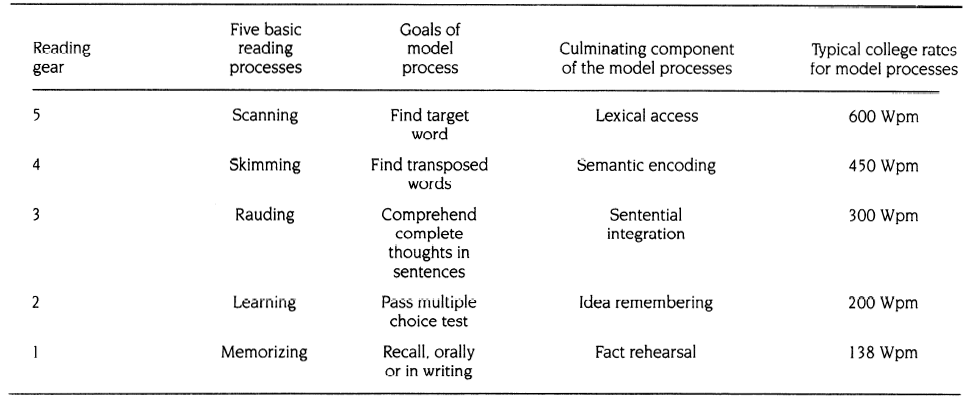
\includegraphics[width=0.8\textwidth]{Pics/gears_list}
\caption{Each gear has its own goal, culminating component, and WPM. \protect\cite{carver_reading_1992}}
\label{fig:ucurve}
\end{figure*}

The goal relies on the reader's intent when reading the text. For instance, the reader could read the text just to find a single word (scanning). The culminating component of a gear, is then the cognitive process that it requires. \textit{Lexical access} is the component used for finding a single word in memory. If the reader's goal changed to finding a certain sentence in the text, such as in skimming, transposed words must be found and the activity would require an additional component; \textit{semantic encoding}. Other than just finding the words, the reader must now determine the meaning of the sentence. In order for the reader to understand the complete thought of a sentence, the \textit{sentential integration} component must be added. These three components together are the requirement for the most basic and most used reading process - \textit{rauding}, also known as \textit{typical reading}. The word comes from a combination of 'auding' and 'reading', as they both share the same underlying comprehension processes. If the goal of reading the text is to learn, e.g., in order to answer a test, the \textit{idea remembering} component is added. In this gear, some words require re-reading and longer time to process. The final gear is focused around remembering the text and uses the \textit{fact rehearsal} component. This gear requires rehearsing the material and memorizing it. 
\citeA{carver_reading_1992} goes on to mention that the best readers shift up and down in gear while reading, based on the difficulty of the material - a term called \textit{process flexibility}. 

By having college students read a text followed by answering two multiple choice tests, as well as judging their own performance, \citeauthor{carver_reading_1992} tested efficiency at different reading rates. It was found that the students were most efficient at rates around 300 WPM - the rauding reading rate. This rate has therefore been referred to as the most optimal reading rate.
%Efficiency was calculated from the product of accuracy and reading rate, and the accuracy was determined through multiple-choice tests as well as self-judgement.

\citeauthor{carver_reading_1992} also mentions the term \textit{cognitive speed}, which acts as a limit of the reading speed. If the reader passes this limit, he will not be able to operate the culminating components successfully, resulting in a poor comprehension. The main concern however for most students is to make the reading speed reach the limit of the cognitive speed.

\citeauthor{carver_reading_1992} describes how \textit{rauding theory} relates to the \textit{schema theory}. Schema theory uses gears 1 and 2, but mainly focuses on how readers learn or memorize text. \citeA{widmayer_schema_2005} presents schema as a set of rules that help processing new information by interpreting and predicting situations occurring in the environment. Specifically for reading, \citeauthor{widmayer_schema_2005} claims that using schema allows learners to process information more effectively while reading. A common reading strategy that incorporates this is making predictions of the text before reading it by for instance reading the titles and looking at the pictures first.

This might indicate that when using schema, readers use skimming or scanning before reading a text, but shift to the memorization and learning gears as soon as they start reading. It also indicated that a complete overview of the text can be relevant in some cases.

%(INSERT REF: Reading for One Second, One Minute, or One Year) compares four different theoretical perspectives in reading, each focusing on a certain style and speed of reading: Rauding, Verbal Efficiency, Schema, and Whole Language.